\documentclass[CMPE]{KGCOEReport}

\usepackage{graphicx}
\usepackage{float}

\newcommand{\classCode}{CMPE 160}
\newcommand{\name}{Chris Larson}
\newcommand{\LabSectionNum}{3}
\newcommand{\LabInstructor}{Miguel Dominguez}

\newcommand{\TAs}{Andrew Ramsey \\ Madeline Mooney \\ Matthew Millar}
\newcommand{\LectureSectionNum}{2}
\newcommand{\LectureInstructor}{Professor Beato}
\newcommand{\exerciseNumber}{11}
\newcommand{\exerciseDescription}{Modeling of Combinational Circuits Using Concurrent and Sequential Statements}
\newcommand{\dateDone}{4/4/18}
\newcommand{\dateSubmitted}{4/11/18}

\begin{document}
\maketitle

\section*{Abstract}
The objective of this exercise was to learn how to write different types of models in VHDL, specifically data flow, structural, and behavioral models. Three different models were used to construct a 74LS153 circuit, two 4:1 multiplexers and simulated in Modelsim using testbenches that were created to ensure the correctness of the models. Each of the different models use the same entity declaration of a dual 4-line to 1-line data multiplexers circuit, and created the same circuit and waveform in the end. The exercise was successful in showing that there are multiple ways to create the same circuit in VHDL, this was shown to be correct as the waveforms of all three models matched each other.

\section*{Design Methodolgy}
 Table 1 shows the functionality of the circuit, DM74LS153. 'L" is equivalent to logic '0', 'H' to logic '1' and 'X' denotes any value.

\begin{table}[H]
	\centering
	\caption{Function Table of DM74LS153}
	\label{tab:Table 1}
	\begin{tabular}{|c|c|c|c|c|c|c|c|}
		\hline
		Select In & Select In & Data In & Data In & Data In & Data In & Strobe & Output\\ \hline
		B & A & C0 & C1 & C2 & C3 &G & Y \\ \hline 
		X & X & X & X & X & X & H & L\\ \hline
		L & L & L & X & X & X & L & L\\ \hline
		L & L & H & X & X & X & L & H\\ \hline
		L & H & X & L & X & X & L & L\\ \hline
		L & H & X & H & X & X & L & H\\ \hline
		H & L & X & X & L & X & L & L\\ \hline
		H & L & X & X & H & X & L & H\\ \hline
		H & H & X & X & X & L & L & L\\ \hline
		H & H & X & X & X & H & L & H\\ \hline
	\end{tabular}
\end{table}

 A dataflow model defines the outputs as a funciton of inputs and is very similar to entering Boolean equations. Using basic outlines for the model that were given, the dataflow model was created using a "with select" statement that assigned a value to an output when the inputs were of a certain value. The dataflow model did not include any propogration delays.  The second model was created using a behavioral model, which is a functional type of modeling that uses an algorithmic approach and is similar to high-level programming. The behavioral model utilized two case statements and two processes, one for each mux, with a propagation delay of 22ns for all inputs to all output. The third model used structural architecture, uses a hierachical approach and interconnects multiple VHDL files to compose a larger system, each of the gates have to be created as separate entities. In the three-level system, there were models for an inverter, 4-input AND< and 4-input OR gates, the inverter had a delay of 4 ns while the other two gates had a delay of 7 ns. These 3 gates were used to create the second level of the system, the 4-to-1 mux which comprised of 5 inverters, 4 AND gates and a single OR gate. The mux was then combined with another mux to create the third-level of the system, the entire circuit. 

\section*{Results and Analysis} 
After all of the models were created a testbench was created to test and ensure the correctness of all three of the models as well as compare the waveforms of each of the models to show that they are the same. A behavioral architecture was created that tested the entity using each of the architecture, and changing the input, and signal values to test for multiple outcomes.Four test were done, two test sets were made shown in Table 2 and 3, and for the third and fourth test the value for 'G' is '1' instead of '0' while everything else stays the same. Table 2 shows the test set that was used for case one and case three but in case three all the values for 'G' are '1' instead of '0'.

\begin{table}[H]
	\centering
	\caption{Test set 1}
	\label{tab:Table 2}
	\begin{tabular}{|c|c|c|c c c c|}
		\hline
		G & B & A & C0 & C1 & C2 & C3 \\ \hline
		0 & 0 & 0 & 0 & 1 & 1 & 1 \\ \hline
		0 & 0 & 0 & 1 & 0 & 0 & 0 \\ \hline
		0 & 0 & 1 & 1 & 0 & 1 & 1 \\ \hline
		0 & 0 & 1 & 0 & 1 & 0 & 0 \\ \hline
		0 & 1 & 0 & 1 & 1 & 0 & 1 \\ \hline
		0 & 1 & 0 & 0 & 0 & 1 & 0 \\ \hline
		0 & 1 & 1 & 1 & 1 & 1 & 0 \\ \hline
		0 & 1 & 1 & 0 & 0 & 0 & 1 \\ \hline
	\end{tabular}
\end{table}

Table 3 shows the test set that was used for case two and case four but in case four all the values for 'G' are '1' instead of '0'. The results for case one is shown in Figure 1, which shows the waveforms for the test case.

\begin{table}[H]
	\centering
	\caption{Test set 2}
	\label{tab:Table 3}
	\begin{tabular}{|c|c|c|c c c c|}
		\hline
		G & B & A & C0 & C1 & C2 & C3 \\ \hline
		0 & 0 & 0 & 0 & 1 & 0 & 1 \\ \hline
		0 & 0 & 1 & 0 & 1 & 0 & 1 \\ \hline
		0 & 1 & 0 & 0 & 1 & 0 & 1 \\ \hline
		0 & 1 & 1 & 0 & 1 & 0 & 1 \\ \hline
		0 & 0 & 0 & 1 & 0 & 1 & 0 \\ \hline
		0 & 0 & 1 & 1 & 0 & 1 & 0 \\ \hline
		0 & 1 & 0 & 1 & 0 & 1 & 0 \\ \hline
		0 & 1 & 1 & 1 & 0 & 1 & 0 \\ \hline
	\end{tabular}
\end{table}

The waveforms in Figure 1-4 show the correct ouputs for the test cases of the models. Figure 1 shows the results for test case one.
\begin{figure}[H]
	\centering
	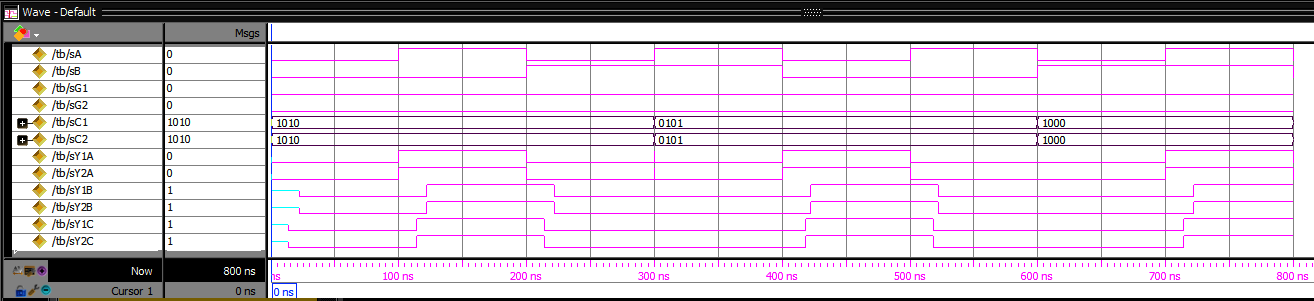
\includegraphics[width=1\textwidth]{ModelSimLab11PT1}
	\caption{Test Case 1}
	\label{fig:Figure 1}
\end{figure}

The results for case two is shown in Figure 2, which shows the waveforms for the test case.

\begin{figure}[H]
	\centering
	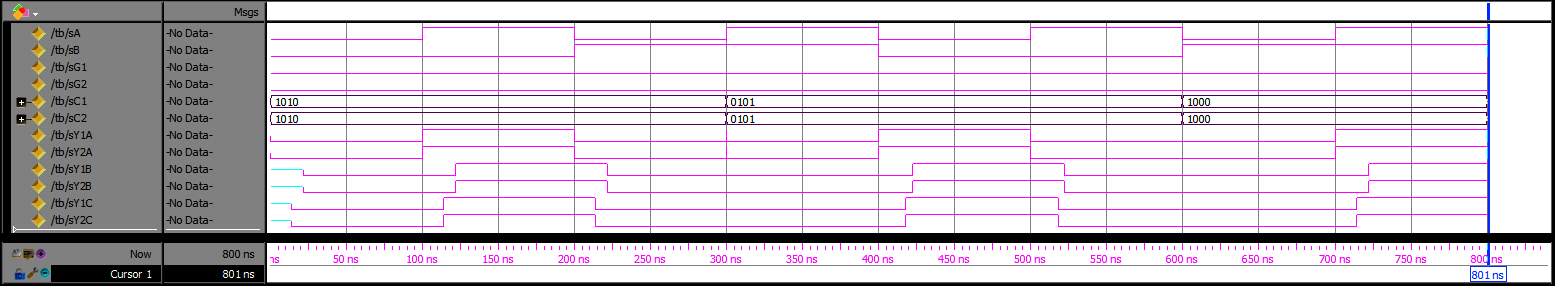
\includegraphics[width=1\textwidth]{ModelSimLab11PT2}
	\caption{Test Case 2}
	\label{fig:Figure 2}
\end{figure}

The results for case three is shown in Figure 3, which shows the waveforms for the test case. The ouputs for this case and case four are flat because when 'G' is at value  '1' the circuit outputs '0' and nothing else.

\begin{figure}[H]
	\centering
	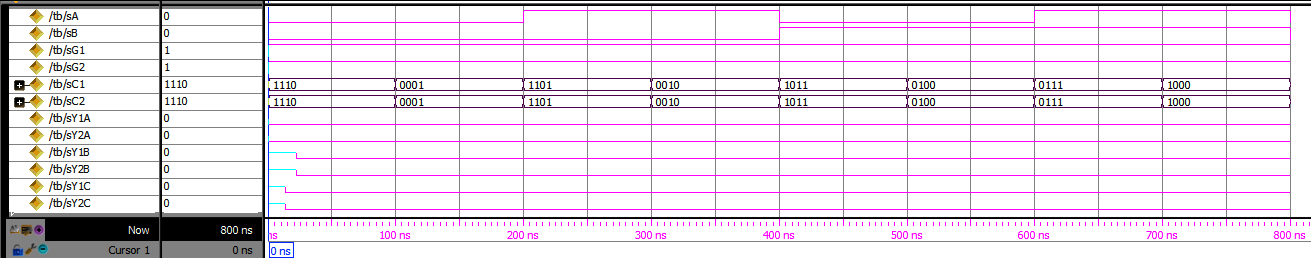
\includegraphics[width=1\textwidth]{ModelSimLab11PT3}
	\caption{Test Case 3}
	\label{fig:Figure 3}
\end{figure}

The results for case one is shown in Figure 4, which shows the waveforms for the test case and similar to case three are zero and flat lined.

\begin{figure}[H]
	\centering
	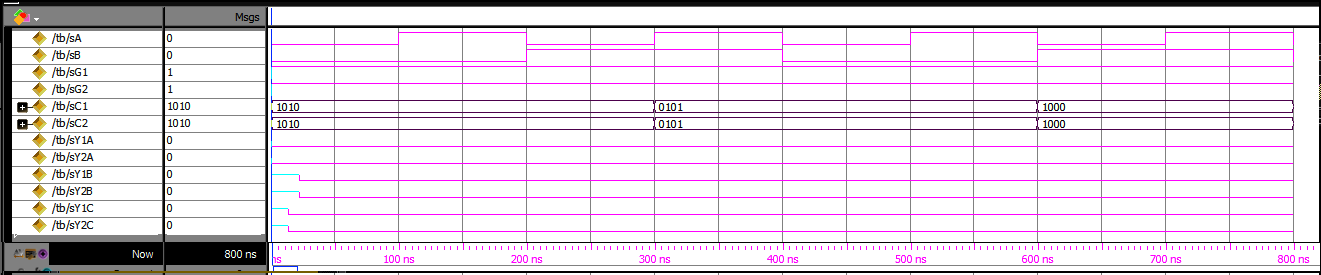
\includegraphics[width=1\textwidth]{ModelSimLab11PT4}
	\caption{Test Case 4}
	\label{fig:Figure 4}
\end{figure}

The results of this exercise were successful as confirmed by the waveforms showing that all three different models output the same waveforms with every single test case, which confirms that the models were written correctly and the test bench was also written correctly. The only difference between the waveforms is the unique propagation delay in each of the models that helps ensure that it is performing correctly.

\section*{Conclusion}
The use of different models such as data flow, behavioral and structural is a key aspect of learning VHDL because it allows for the user to create different solutions that might be more efficient than another model. The use of waveforms to ensure that the models were the same in function allows for confirming models that are created work proper or that, similar to this exercise perform the same as another model. The exercise was successful in showing that there are multiple ways to create the same circuit as well as showing that waveforms are an easy way to compare the outputs of the models to ensure that the models function the same. Testbenches are key to creating the waveforms and testing specific cases that may arise or all of the different situations the circuit could encounter.

\section*{Questions}
A delta delay is a very very tiny amount of delay. It is useful for scheduling and ordering the events that occur during the simulation time since in VHDL events happen concurrent or at the same time. Delta delay allows for events to happen at the same "time" but still in an order that is not random. 


\begin{figure}[H]
	\centering
	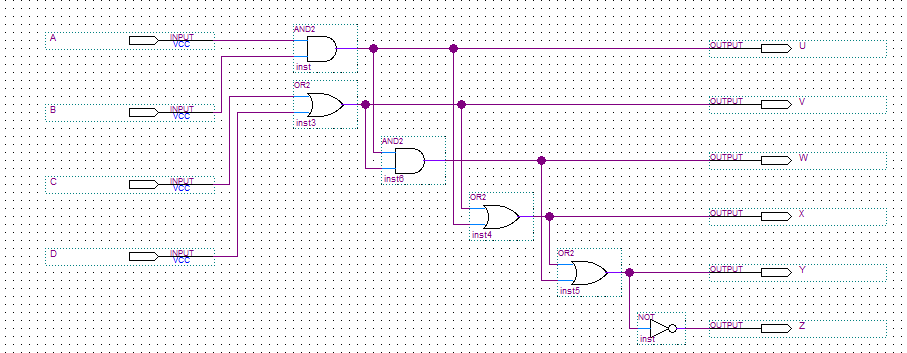
\includegraphics[width=1\textwidth]{QuartusLab11Q}
	\caption{Question Quartus}
	\label{fig:Figure 5}
\end{figure}

\end{document}